\documentclass[xetex,mathserif,serif]{beamer}
\usepackage{polyglossia}
\setdefaultlanguage[babelshorthands=true]{russian}
\usepackage{minted}
\usepackage{tabu}
\usepackage{moresize}

\useoutertheme{infolines}

\usepackage{fontspec}
\setmainfont{FreeSans}
\newfontfamily{\russianfonttt}{FreeSans}

\definecolor{links}{HTML}{2A1B81}
\hypersetup{colorlinks,linkcolor=,urlcolor=links}

\usepackage{beamerthemesplit} 
\usepackage{wrapfig} 
\usepackage{verbatim} 
\usepackage{pdfpages} 
\usepackage{amsmath} 
\usepackage{cmap}
\usepackage{array} 
\usepackage{amsmath} 
\usepackage{tikz} 
\usepackage{multirow} 
\usepackage[noend]{algpseudocode} 
\usepackage{algorithm} 
\usepackage{algorithmicx} 
\usetikzlibrary{shapes,arrows} 
\usetikzlibrary{calc}
\usepackage{fancyvrb} 
\usepackage{tikz} 
\usepackage{pgfplots} 
\usepackage{sidecap} 
\usepackage{soul}
\usepackage{xcolor}
\usepackage{tabu}
\usepackage{zref-savepos}
\usepackage{colortbl}
\usepackage[normalem]{ulem}
\pgfplotsset{compat=1.9} 
\newtheorem{rutheorem}{Теорема} 
\newtheorem{ruproof}{Доказательство} 
\newtheorem{rudefinition}{Определение} 
\newtheorem{rulemma}{Лемма} 
\beamertemplatenavigationsymbolsempty 

\newcounter{NoTableEntry}
\renewcommand*{\theNoTableEntry}{NTE-\the\value{NoTableEntry}}

\newcommand*{\strike}[2]{%
	\multicolumn{1}{#1}{%
		\stepcounter{NoTableEntry}%
		\vadjust pre{\zsavepos{\theNoTableEntry t}}% top
		\vadjust{\zsavepos{\theNoTableEntry b}}% bottom
		\zsavepos{\theNoTableEntry l}% left
		\hspace{0pt plus 1filll}%
		#2% content
		\hspace{0pt plus 1filll}%
		\zsavepos{\theNoTableEntry r}% right
		\tikz[overlay]{%
			\draw
			let
			\n{llx}={\zposx{\theNoTableEntry l}sp-\zposx{\theNoTableEntry r}sp-\tabcolsep},
			\n{urx}={\tabcolsep},
			\n{lly}={\zposy{\theNoTableEntry b}sp-\zposy{\theNoTableEntry r}sp},
			\n{ury}={\zposy{\theNoTableEntry t}sp-\zposy{\theNoTableEntry r}sp}
			in
			(\n{llx}, \n{lly}) -- (\n{urx}, \n{ury})
			;
		}% 
	}%
}

\title[MIRF]{Medical Images Research Framework} 
\institute[SPbSU]{Saint-Petersburg State University \\
	Software Engineering chair} 

\author[Yurii Litvinov]{Sabrina Musatyan \\
	\and
	Alexander Lomakin \\
	\and
	Angelina Chizhova \\
	\and
	{\bfseries Yurii Litvinov}
	}

\date{03.08.2019} 

\begin{document} 
\definecolor{red}{RGB}{255,0,0} 

\begin{frame}
	\begin{center} 
		{
\includegraphics[width=1cm]{pictures/SPbGU_Logo.png}} 
	\end{center}
	\titlepage
\end{frame}


\begin{frame}
     \frametitle{Motivation}
        \begin{figure}[b]
             \centering
             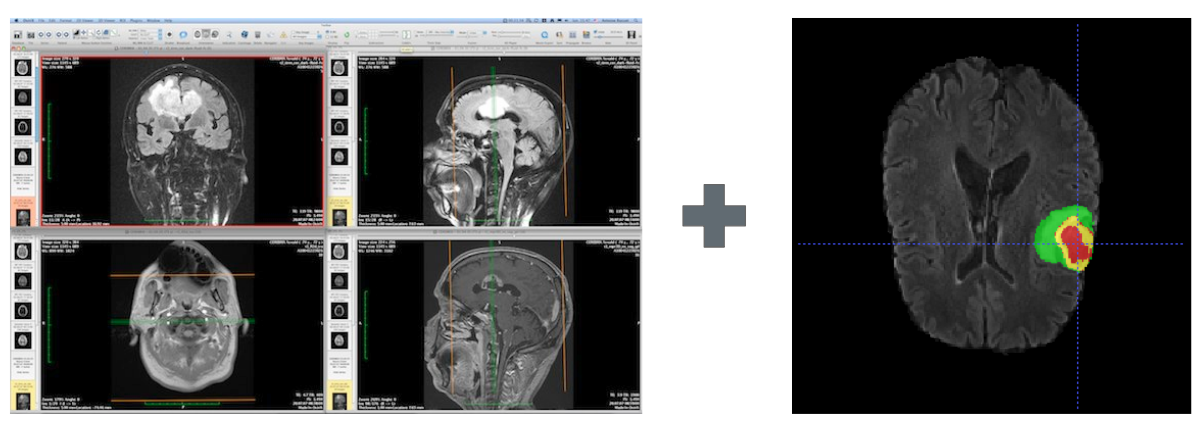
\includegraphics[width=12cm]{pictures/brainseg.png}
         \end{figure}
\end{frame}

\begin{frame}
    \frametitle{Related work}
    \begin{figure}[b]
        \centering
        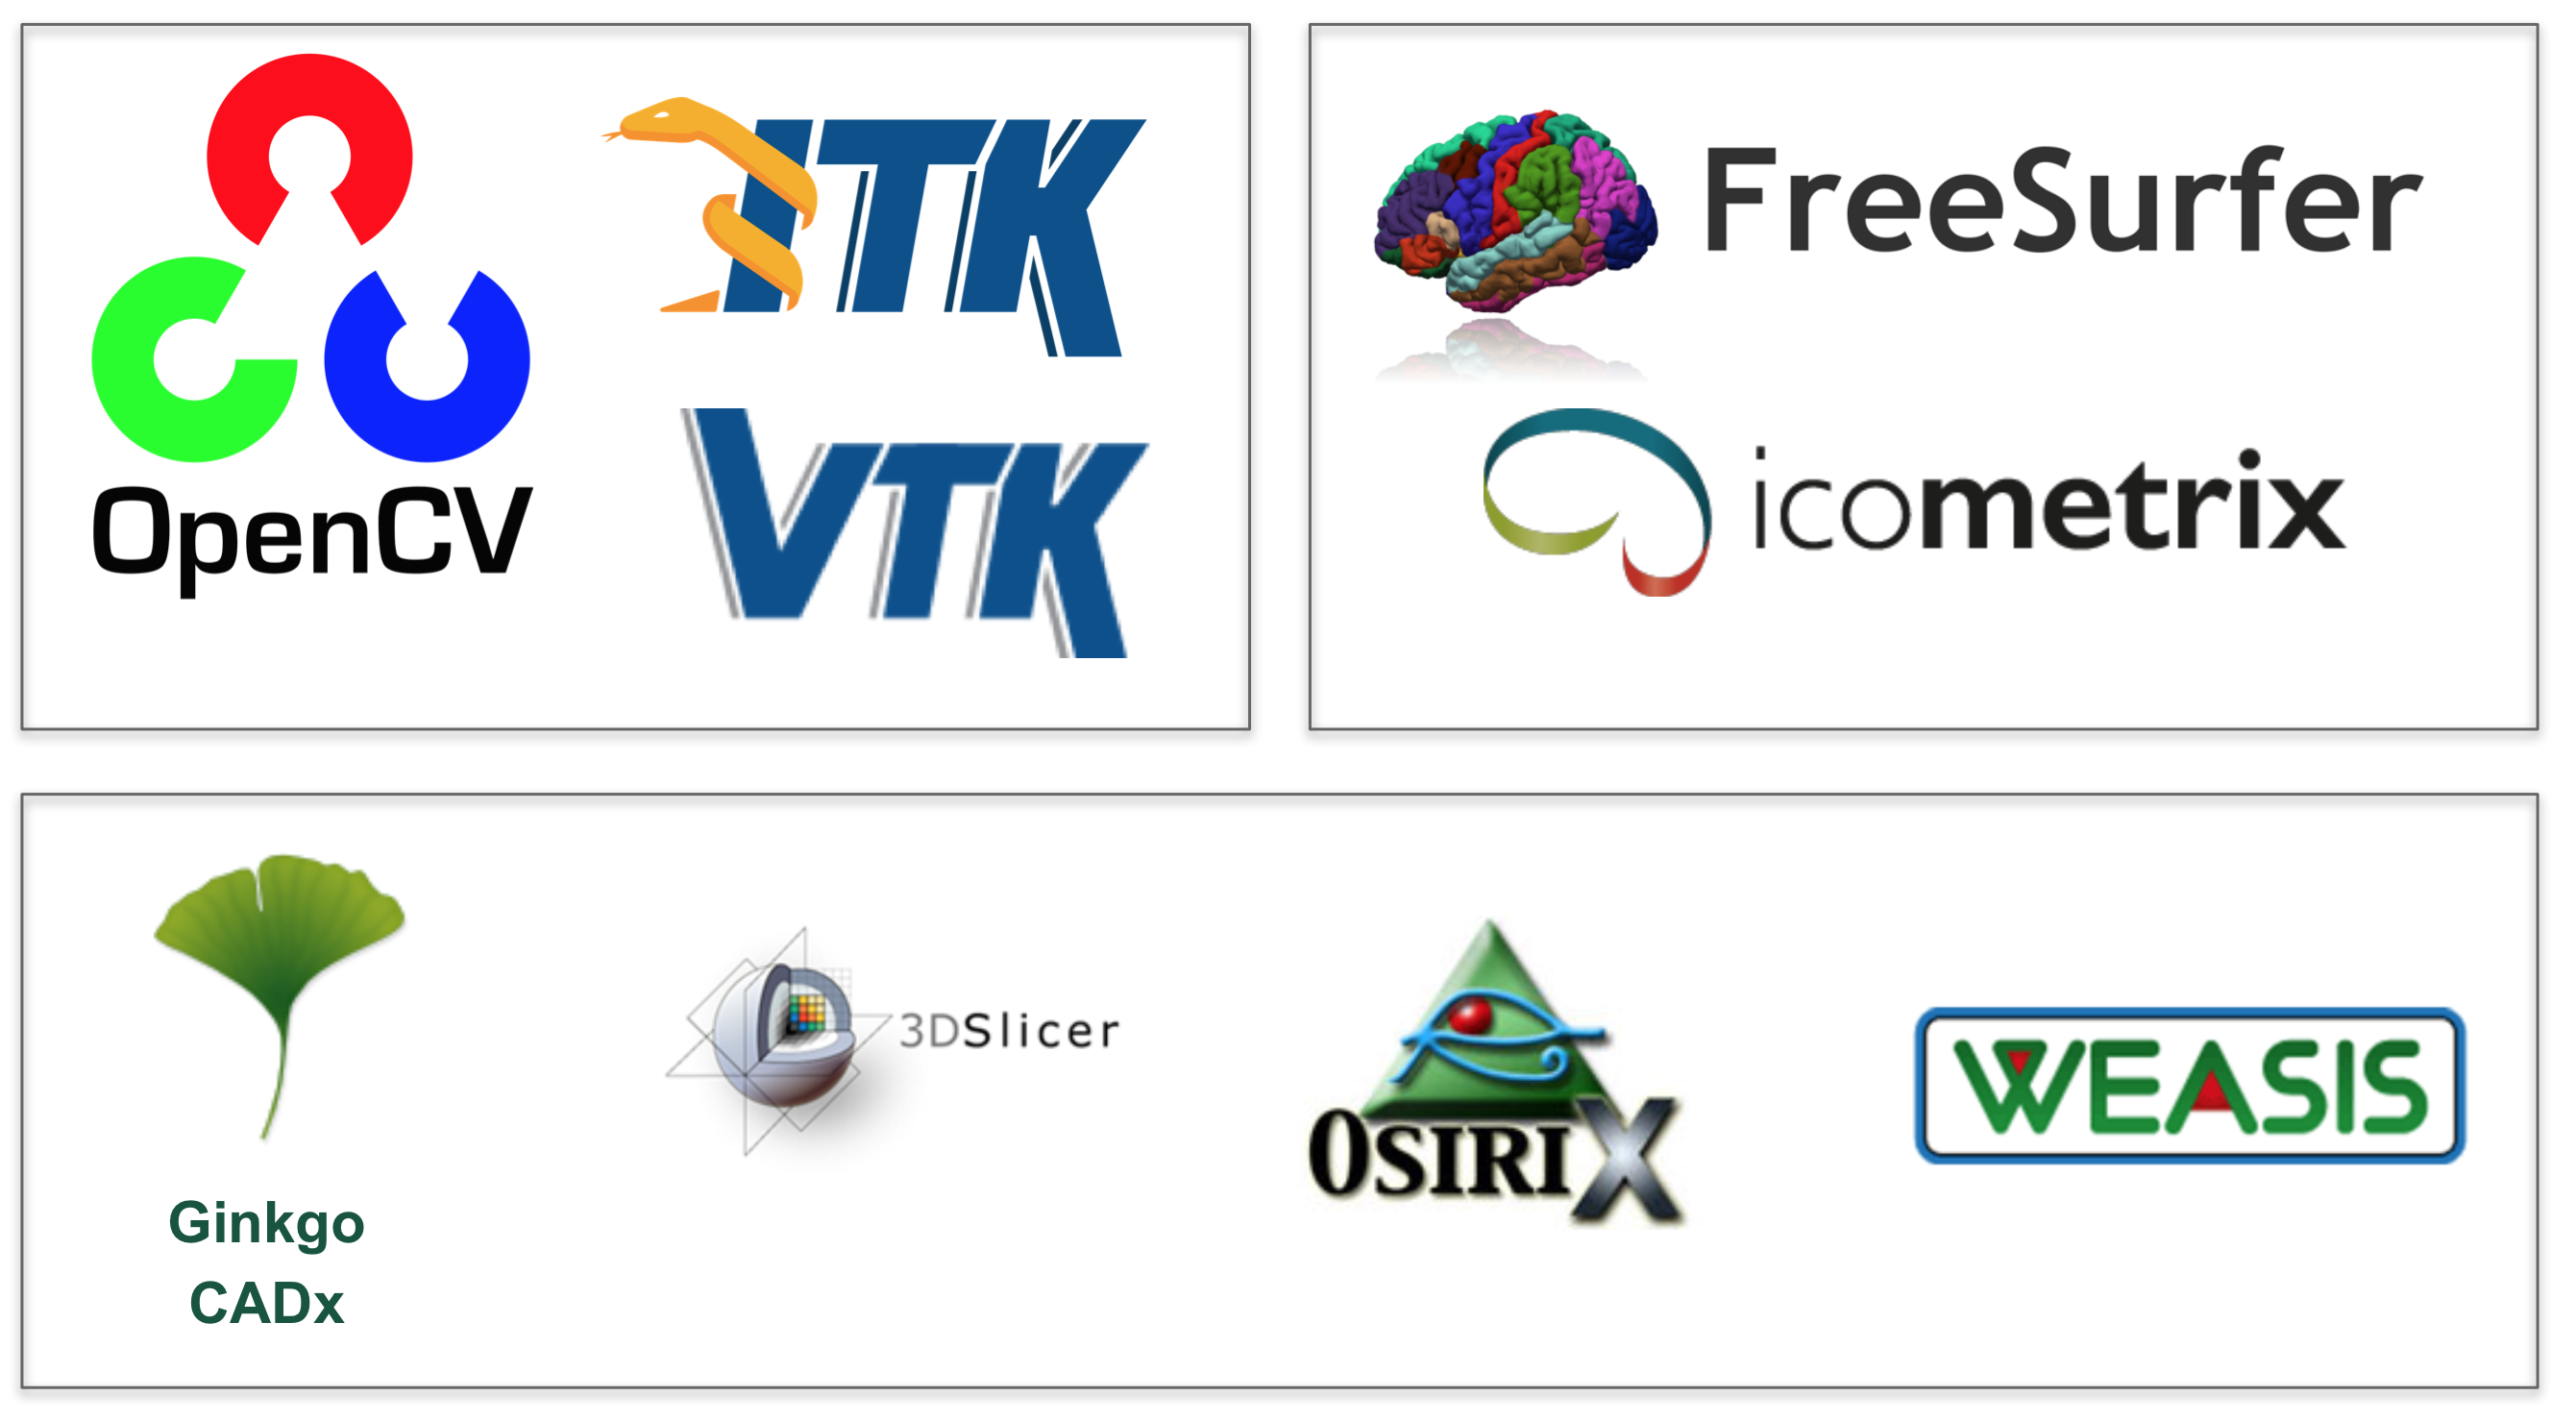
\includegraphics[width=12cm]{pictures/overview.png}
    \end{figure}
\end{frame}
  
 \begin{frame}
     \frametitle{MITK vs MIRF}
     \begin{tabular}{p{5cm} p{6cm}}
        \begin{figure}[b]
             \centering
             
\includegraphics[width=4.5cm]{pictures/mitk.png}  
         \end{figure}
         \begin{itemize}
             \item C++
             \item Requires integration into its own infrastructure
             \item Many good plugins  for medical images
         \end{itemize}
         &
         \begin{figure}[b]
             \centering
             
\includegraphics[width=4.0cm]{pictures/mirf.png}  
         \end{figure}
         \begin{itemize}
             \item Kotlin
             \item Can be integrated into existing applications
             \item Cross-platform and supports mobile apps
         \end{itemize}
     \end{tabular}
 \end{frame}
 
\begin{frame}
     \frametitle{MIRF architecture}
        \begin{figure}[b]
             \centering
             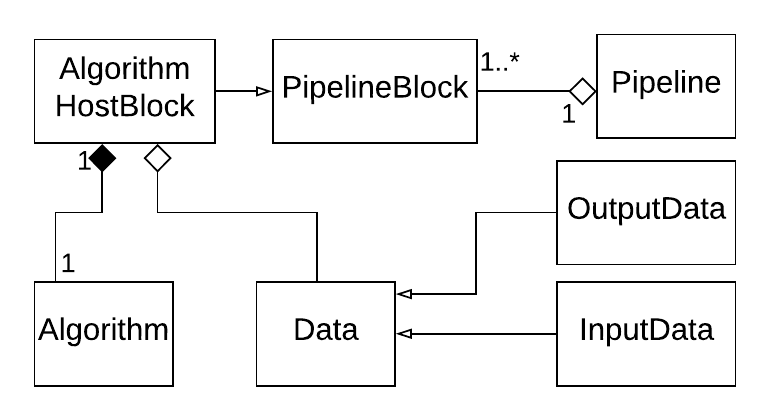
\includegraphics[width=12cm]{pictures/pipe.png}
         \end{figure}
\end{frame}
 
\begin{frame}
    \frametitle{Supported image formats}
        \begin{itemize}
            \item Common intermediate representation
            \item Supported formats:
                    \begin{itemize}
                         \item DICOM
                         \item NIfTI
                         \item MHD (from ITK)
                     \end{itemize}
         \end{itemize}
 \end{frame}

  \begin{frame}
     \frametitle{Report generation}
        \begin{figure}[b]
             \centering
             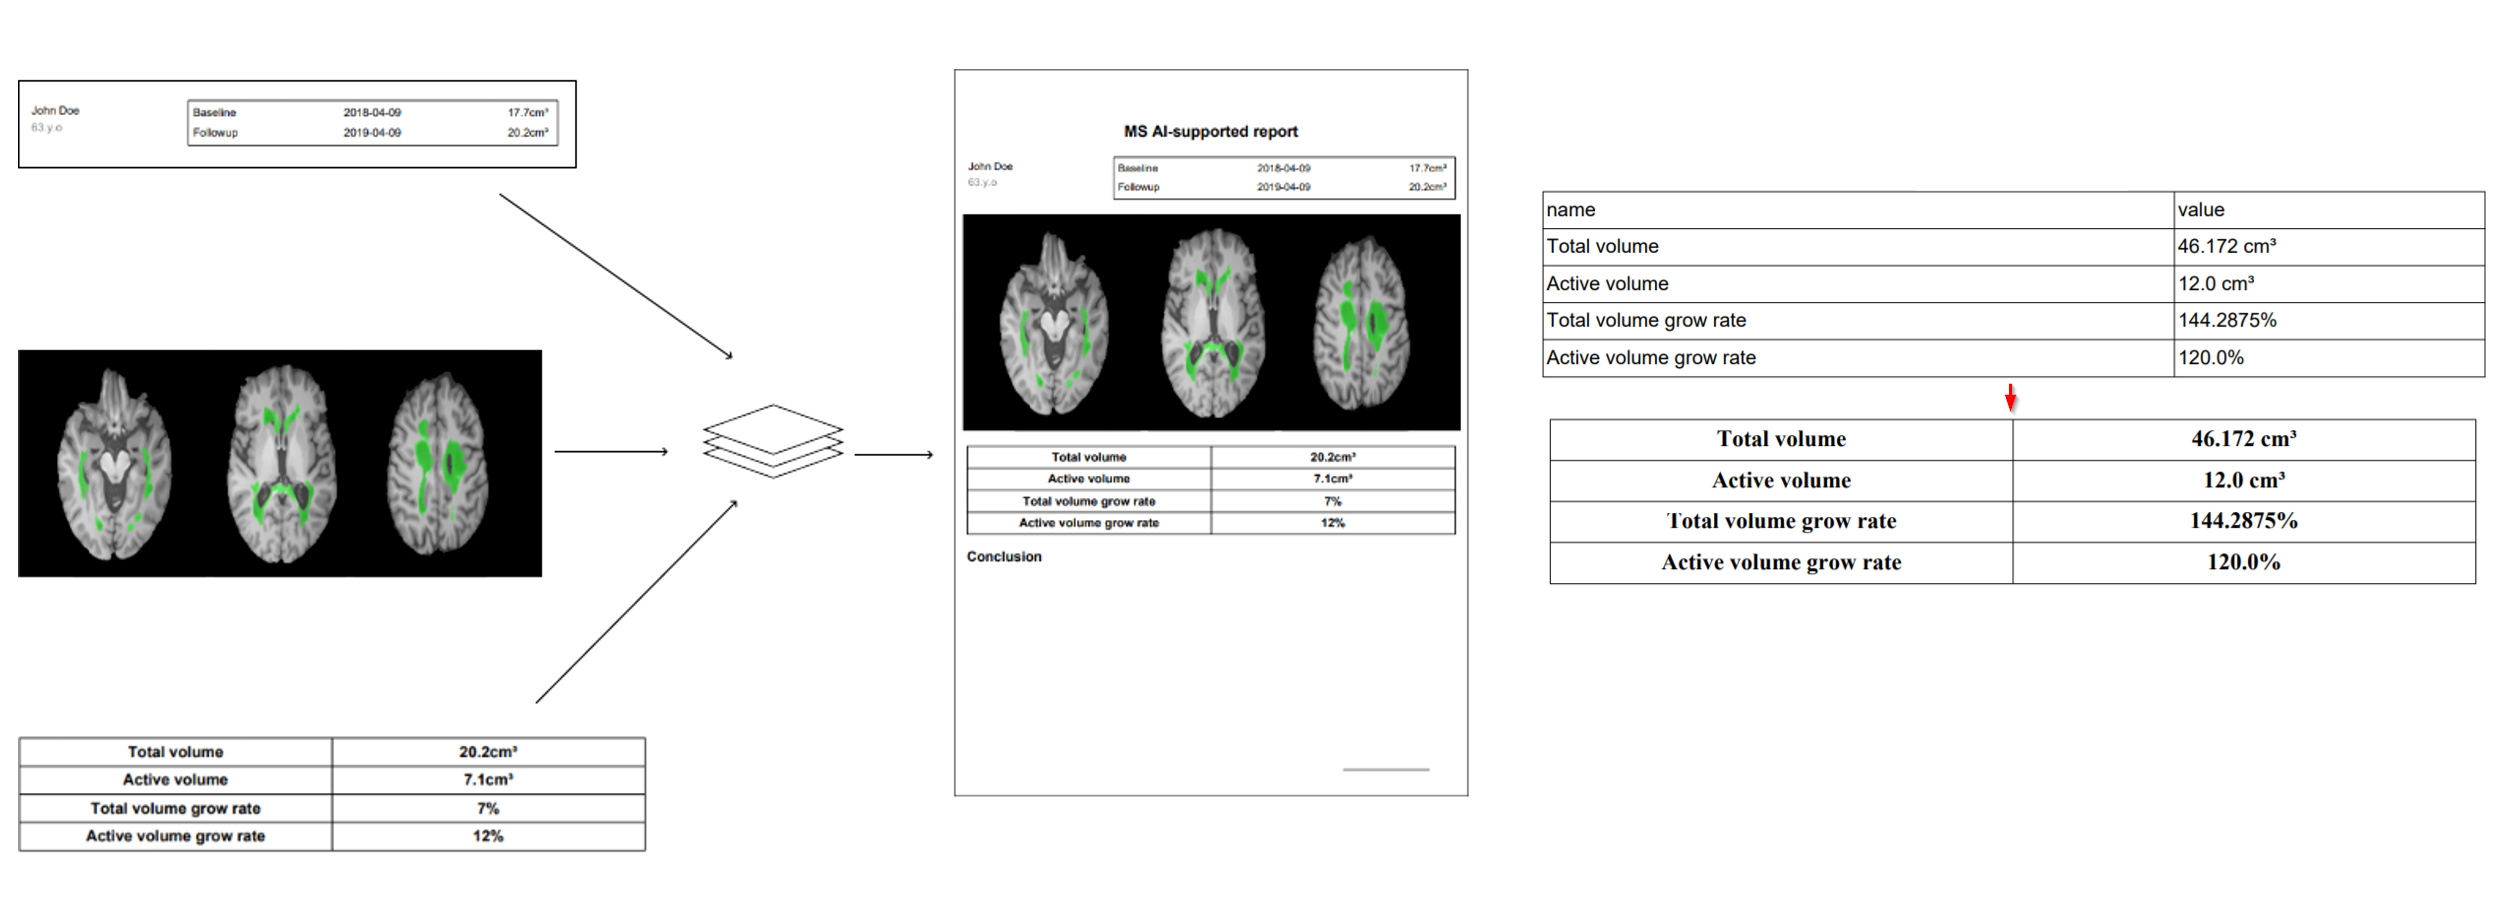
\includegraphics[width=12cm]{pictures/reports.png}
         \end{figure}
 \end{frame}
 
 \begin{frame}
     \frametitle{Tensorflow integration}
        \begin{itemize}
             \item Java API for Tensorflow
             \item Wrapper blocks for pre-learned models
         \end{itemize}
 \end{frame}
 
   \begin{frame}
     \frametitle{Example: brain tumor analysis}
    \begin{tabular}{p{5cm} p{7cm}}
        \begin{figure}[b]
             \centering
             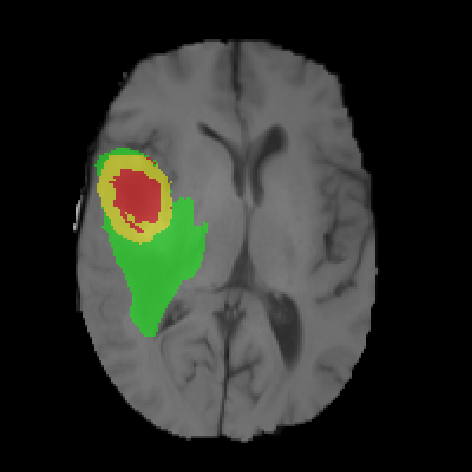
\includegraphics[width=3.5cm]{pictures/brain_seg.png}
         \end{figure}
         Various tumor tissues: necrotic core (red),
         tumor site (yellow), edema (green)
         &
         \begin{figure}[b]
             \centering
             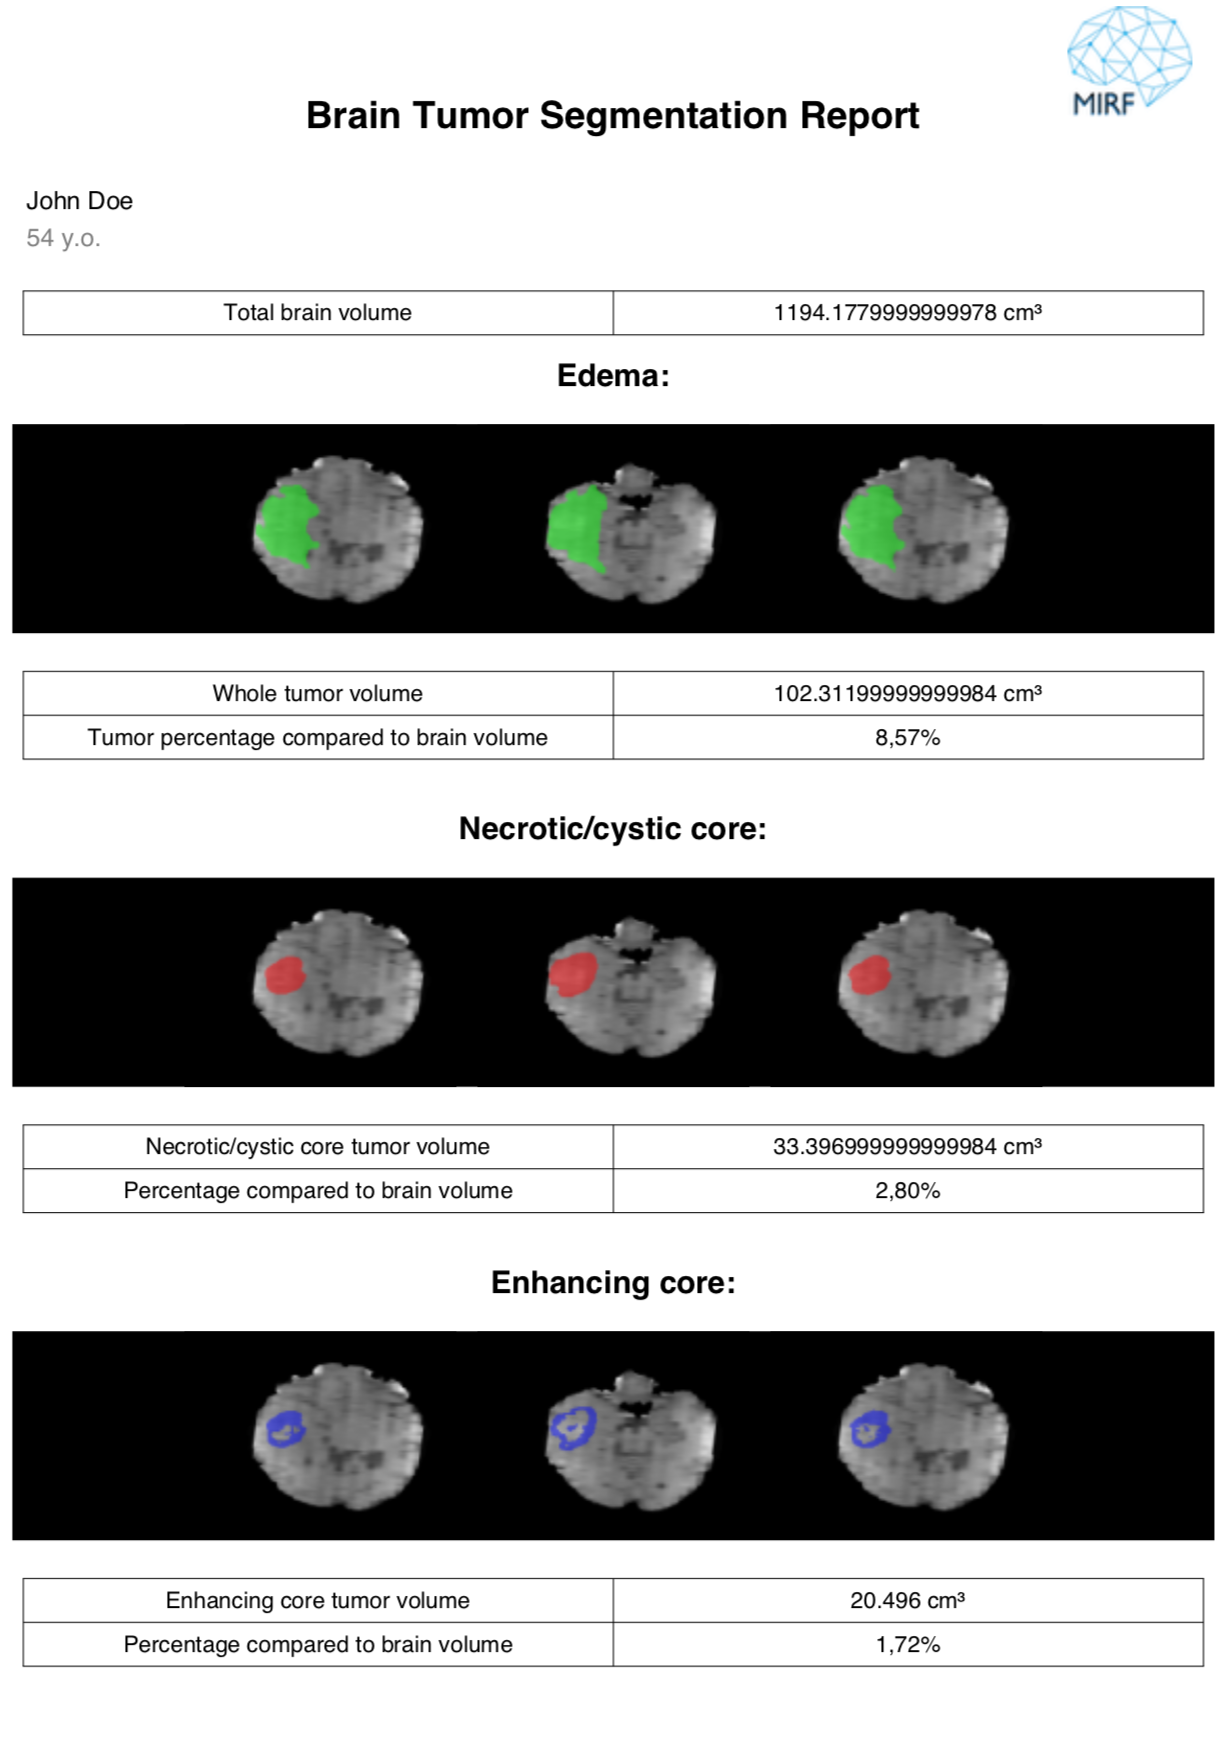
\includegraphics[width=4.8cm]{pictures/pdf.png}
         \end{figure}
     \end{tabular}
 \end{frame}
 
  \begin{frame}
     \frametitle{Example: brain tumor analysis}
        \begin{figure}
             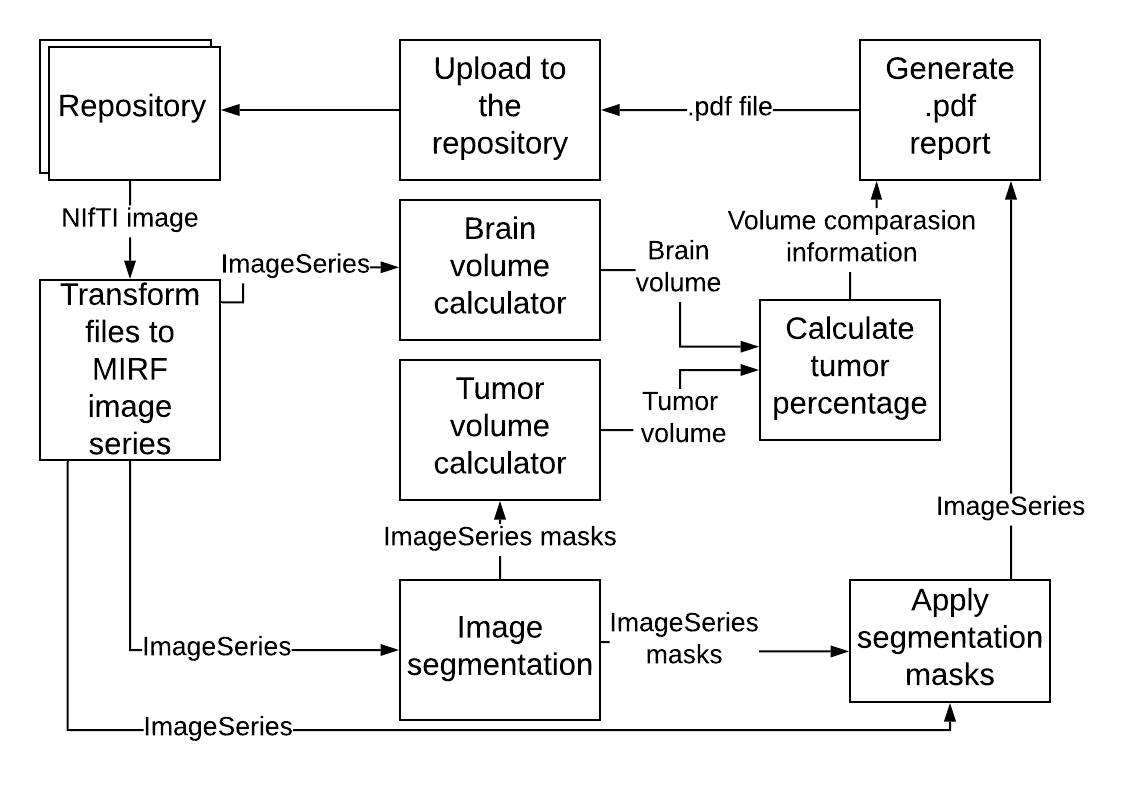
\includegraphics[width=11cm]{pictures/brainsch.png}
         \end{figure}
 \end{frame}

 
  \begin{frame}
     \frametitle{Example: multiple sclerosis}
        \begin{figure}
             \includegraphics[width=5cm]{pictures/mirfms.png}
         \end{figure}
 \end{frame}

   \begin{frame}
     \frametitle{Android integration}
        \begin{itemize}
             \item Example: skin cancer diagnosis using phone camera
                 \begin{tabular}{p{5cm} p{5cm}}
        \begin{figure}[b]
             \centering
             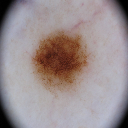
\includegraphics[width=2.0cm]{pictures/benign.png}
         \end{figure}
         Benign mole
         &
         \begin{figure}[b]
             \centering
             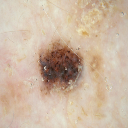
\includegraphics[width=2.0cm]{pictures/malig.png}
         \end{figure}
         Malignant mole
     \end{tabular}
             \item Separate MIRF build for Android
         \end{itemize}
 \end{frame}
 
\end{document}